\begin{figure*}
  \centering
  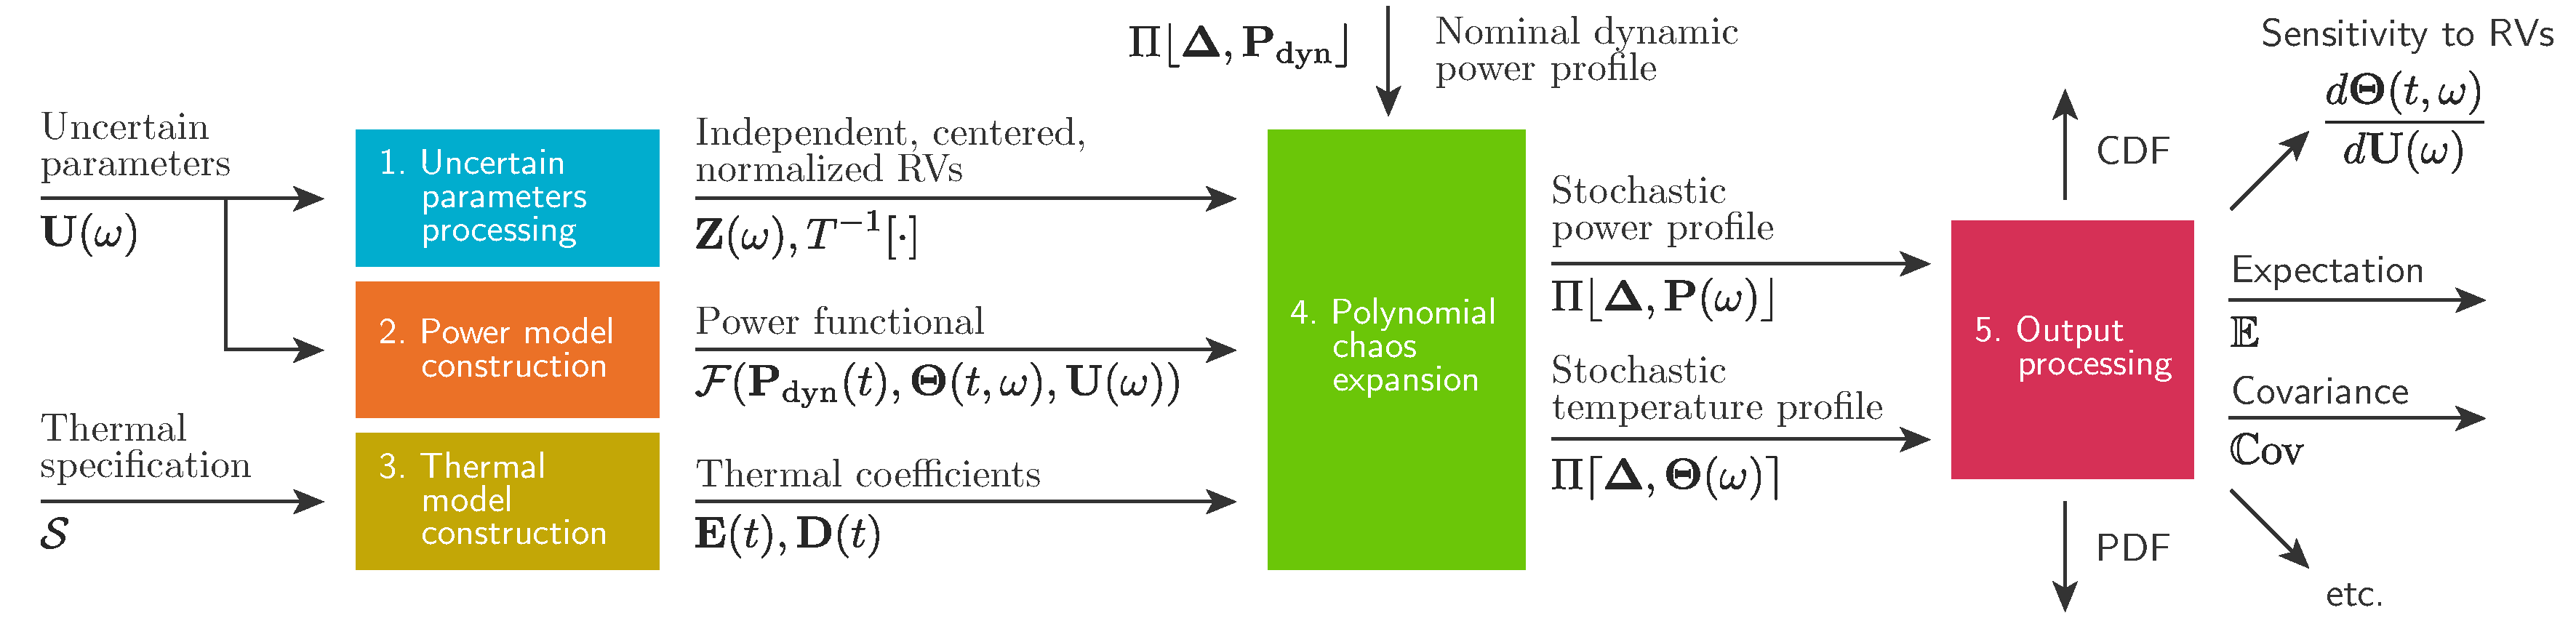
\includegraphics[width=0.9\textwidth]{include/assets/algorithm.pdf}
  \vspace{-0.7em}
  \caption{The structure of the proposed framework.}
  \flabel{algorithm}
  \vspace{-1.6em}
\end{figure*}

Consider a heterogeneous multiprocessor system that consists of $\cores$ processing elements and is equipped with a thermal package. The processing elements are the active components of the system defined at the intended level of granularity (ALUs, caches, registers, etc.). Let $\system$ be a thermal specification of the system defined as a collection of temperature-related information: (a) the floorplans of the active layers of the chip; (b) the geometry of the thermal package; (c) the thermal parameters of the materials that the chip and package are made of. In this work, $\system$ is assumed to be deterministic. In addition, the system depends on a set of uncertain parameters, denoted by $\vU(\o)$, which manifest themselves in the deviation of the actual power dissipation from nominal values and, consequently, in the deviation of temperature from the one corresponding to the nominal power dissipation.

In order to quantify the system, we introduce the following definition. A system profile of a quantity $Q$ over a time interval $\period$ is a tuple $(\part, \m{Q})$ where $\part = \{ 0 = \t_0 < \dotsc < \t_{\steps} = \period \}$ is a partition of $\period$ into $\steps$ subintervals $\{ \dt_i = \t_i - \t_{i - 1} \}_{i = 1}^{\steps}$, and $\m{Q} \in \real^{\cores \times \steps}$ is a real matrix that captures the values of $Q$ for all $\cores$ processing elements at either beginning or end of all $\steps$ time intervals. In the former case, the profile is denoted by $\profB{\m{Q}}$, and by $\profE{\m{Q}}$ in the latter. In particular, we are interested in the power profile $\profP$ and, following it, temperature profile $\profT$ (hereafter, $P$ stands for power and $\T$ for temperature). Since the system is stochastic, we shall distinguish between deterministic (nominal) and stochastic power and temperature profiles. In the stochastic case, $\profP{\o}$ and $\profT{\o}$ contain \rvs.

In this work, we aim to develop an UQ framework for power-temperature analysis (PTA) of multiprocessor systems where the power dissipation and temperature are unknown due to the dependency on the set of uncertain parameters $\vU(\o)$. The framework should be based on (a) a high-level thermal specification of the platform $\system$; (b) probability laws (marginal distributions) and a correlation structure (a covariance matrix) of $\vU(\o)$ (\sref{uncertain-parameters}); (c) a model of the power dissipation as a (possibly implicit) function of $\vU(\o)$ (\sref{power-model}). Given a nominal dynamic power profile of the system $\profPdyn$, the framework should deliver the corresponding stochastic power $\profP{\o}$ and temperature $\profT{\o}$ profiles with a desired level of accuracy and a low computational cost.
